\section{Pipeline}

\tikzstyle{process} = [rectangle, rounded corners, minimum width=2cm, minimum height=1cm,text centered, draw=black, fill=gray!50]

\begin{figure}[h]
    \centering
    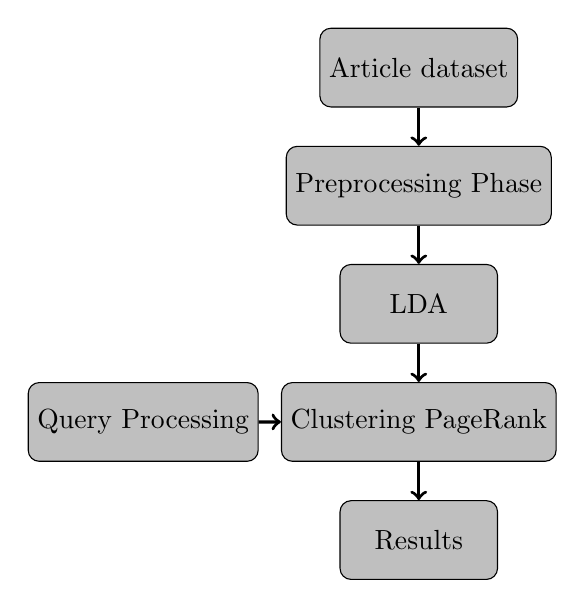
\begin{tikzpicture}[node distance=1.5cm]
    %\draw[step=1cm,gray,very thin] (-8,-8) grid (8,8);
	\node (Dataset) [process] {Article dataset};
	\node (Cleaning)[process, below of=Dataset] {Preprocessing Phase};
	\node (Training) [process, below of=Cleaning] {LDA};
	\node (Cluster PR) [process, below of=Training] {Clustering PageRank};
	\node (Query) at (-3.5, -4.5) [process] {Query Processing};
	\node (Result) [process, below of=Cluster PR] {Results};
	\draw [->, very thick] (Dataset) edge (Cleaning); 
	\draw [->, very thick] (Cleaning) edge (Training);
	\draw [->, very thick] (Training) edge (Cluster PR);
	\draw [->, very thick] (Cluster PR) edge (Result);
	\draw [->, very thick] (Query) edge (Cluster PR);
\end{tikzpicture}
	\caption{Pipeline}
    \label{fig:pipeline}
\end{figure}
The pipeline of our framework is divided into five phases which are displayed in \autoref{fig:pipeline}. \todo[inline]{???? how does that go together???	confusing structure }

\subsection{Article dataset}
We have a dataset consisting of articles from the media group Nordjyske. Their primary focus is to maintain a variety of local newspapers within the North Jutland region of Denmark. 
The data ranges from 2017-2019, where a total of $\sim$270.000 articles have been extracted from their database.

\subsection{Preprocessing Phase}
The extracted articles use the format:
\begin{itemize}
	\item id
	\item headline
	\item body
\end{itemize}
When training the LDA model, we concatenate the \emph{headline} and \emph{body} for simplicity. \todo[inline]{this sentence needs to be moved to another section, it does not match the subsection}
The preprocessing phase is described in further detail in \autoref{subsec:prepro}.
This phase applies different \gls{NLP} methods \todo[inline]{DETAILS!} to simplify the dataset and remove redundant information.
After the preprocessing phase, we are left with $\sim$130.000 articles.

\subsection{LDA}
We apply the \acrfull{lda} to the dataset to generate topic clusters based on the content of the articles. 
We describe the investigation and selection of hyper parameters in \autoref{subsec:lda}. 
After the model has been trained, we have a document-topic distribution matrix $\theta$ and a topic-word distribution matrix $\beta$.
$\theta$ will be used as clusters in the next phase.

\subsection{Cluster-based PageRank}
In this phase, we apply cluster-based random walk, described in \autoref{sec:cluster_pagerank}, to the articles and clusters given in the \gls{lda} phase.
The algorithm yields a prioritized list of articles based on the query provided.


\subsection{Query Preprocessing}
The query \todo[inline]{basics missing I assume we’re talking about keywords} given to the search algorithm is stemmed and turned into a list of words. 
This list of words are then queried against LDA to check which cluster each word belongs to.
Lastly it is transformed into a personalization vector to use within the cluster-based PageRank.
